\documentclass[10pt,a4paper,twoside]{article}
% The following LaTeX packages must be installed on your machine: amsmath, authblk, bm, booktabs, caption, dcolumn, fancyhdr, geometry, graphicx, hyperref, latexsym, natbib

% Please make sure that spp.dat (supplied with this template) is in your working directory or path
\input{spp.dat}

%  Editorial staff will uncomment the next line
% \providecommand{\artnum}[0]{XX-XX}
% \renewcommand{\articlenum}[0]{SPP-\the\year-\artnum-}

\begin{document}

%--------------------------------------------------
%  Fill in the paper's title in Sentence case
%  Titles beginning with articles (A, An, The) are discouraged
%--------------------------------------------------
\title{\TitleFont Article template for submissions to the Proceedings of the Samahang Pisika ng Pilipinas Physics Conference}


%--------------------------------------------------
% For TWO authors with the same affiliation please use this block
% Or Please use the other author block templates
%--------------------------------------------------
\author[*\negthickspace]{Author M.~Surname}
\author[ ]{Bauthor D.~Surname~III
\lastauthorsep}
\affil[ ]{Department of Science, XXX University, Country}
\affil[*]{\corremail{amsurname@university.edu} }

%--------------------------------------------------
%  For three or more authors with the same affiliation please use this block
%--------------------------------------------------

% \author[*]{Author M.~Surname\authorsep}
% \author[ ]{Bauthor D.~Surname~Jr.\authorsep}
% \author[ ]{Cauthor D.~Surname~III\lastauthorsep}
% \affil[ ]{Department of Science, XXX University, Country}
% \affil[*]{\corremail{amsurname@university.edu} }

%--------------------------------------------------
%  For authors with different affiliations please use the following block
%--------------------------------------------------
% \author[1*]{Author M.~Surname\authorsep}
% \author[2]{Bauthor D.~Surname~Jr.\authorsep}
% \author[1,2]{Coauthor G.~Surname~III\authorsep}
% % !!! Please take note that the last author separation is \lastauthorsep instead of \authorsep
% \author[3]{Dauthor G.~Surname\lastauthorsep}
% \affil[1]{Department of Physics, DD University, Country}
% \affil[2]{Department of Science, XX University, Country}
% \affil[3]{Physics Institute, Country}
% \affil[*]{\corremail{amsurname@university.edu} }


\begin{abstract}
\noindent
%--------------------------------------------------
% Include abstract and keywords here
%--------------------------------------------------
Perspiciatis unde omnis iste natus error sit voluptatem accusantium doloremque laudantium, totam rem aperiam, eaque ipsa quae ab illo inventore veritatis et quasi architecto beatae vitae dicta sunt explicabo. Nemo enim ipsam voluptatem quia voluptas sit aspernatur aut odit aut fugit, sed quia consequuntur magni dolores eos qui ratione voluptatem sequi nesciunt. Neque porro quisquam est, qui dolorem ipsum quia dolor sit amet, consectetur, adipisci velit, sed quia non numquam eius modi tempora incidunt ut labore et dolore magnam aliquam quaerat voluptatem. Ut enim ad minima veniam, quis nostrum exercitationem ullam corporis suscipit laboriosam, nisi ut aliquid ex ea commodi consequatur? Quis autem vel eum iure reprehenderit qui in ea voluptate velit esse quam nihil molestiae consequatur, vel illum qui dolorem eum fugiat quo voluptas nulla pariatur?

\keywords{keyword 1, keyword 2}

\end{abstract}

\maketitle
\thispagestyle{titlestyle}


%--------------------------------------------------
% the main text of your paper begins here
%--------------------------------------------------
\section{Introduction}\label{sec:intro}
This is the template for articles submitted to the Samahang Pisika ng Pilipinas Physics Congress. Using the included BibTeX template one can cite articles \cite{articlekey}, arXiv preprints \cite{preprintkey}, books \cite{bookkey}, and conference proceedings \cite{proceedingskey,proceedingskey1,proceedingskey2}. It is preferred to insert citations before punctuation \cite{articlekey,preprintkey}. Sections, figures, and tables are referred to by the usual \textbackslash{\ttfamily{ref}}\{...\} command (as seen in Section \ref{sec:intro}).

Use the equation environment
\begin{verbatim}
\begin{equation}\label{eq:law2}
  \vec{F} = m \vec{a}.
\end{equation}	 
\end{verbatim}
to display equations
\begin{equation}\label{eq:law2}
		\vec{F} = m \vec{a} + \nu \bm\sigma.
\end{equation}
The {\ttfamily bm} package allows the use of bold face Greek letters: \textbackslash {\ttfamily bm}\textbackslash {\ttfamily sigma}. Equations are referred in text by the command \textbackslash{\ttfamily eqref}\{{\ttfamily eq:law2}\} as we do here \eqref{eq:law2}.
Longer equations may use the align environment
\begin{verbatim}
\begin{align}
\vec{F} & = \vec{F}_1 + \vec{F}_2  + \vec{F}_3 \nonumber\\
        &\quad + \vec{F}_4 + \vec{F}_5  + \vec{F}_6 \nonumber\\
        &\qquad + \vec{F}_7 + \vec{F}_8 + \vec{F}_9.
\end{align}
\end{verbatim}
to get
\begin{align}
\vec{F} & = \vec{F}_1 +  \vec{F}_2  +  \vec{F}_3  \nonumber \\
 &\quad + \vec{F}_4 +  \vec{F}_5  +  \vec{F}_6  \nonumber \\
 &\qquad + \vec{F}_7 + \vec{F}_8 + \vec{F}_9.
\end{align}

Ed ut perspiciatis unde omnis iste natus error sit voluptatem accusantium doloremque laudantium, totam rem aperiam, eaque ipsa quae ab illo inventore veritatis et quasi architecto beatae vitae dicta sunt explicabo. Nemo enim ipsam voluptatem quia voluptas sit aspernatur aut odit aut fugit, sed quia consequuntur magni dolores eos qui ratione voluptatem sequi nesciunt. Neque porro quisquam est, qui dolorem ipsum quia dolor sit amet, consectetur, adipisci velit, sed quia non numquam eius modi tempora incidunt ut labore et dolore magnam aliquam quaerat voluptatem. Ut enim ad minima veniam, quis nostrum exercitationem ullam corporis suscipit laboriosam, nisi ut aliquid ex ea commodi consequatur? Quis autem vel eum iure reprehenderit qui in ea voluptate velit esse quam nihil molestiae consequatur, vel illum qui dolorem eum fugiat quo voluptas nulla pariatur? ed ut perspiciatis unde omnis iste natus error sit voluptatem accusantium doloremque laudantium, totam rem aperiam, eaque ipsa quae ab illo inventore veritatis et quasi architecto beatae vitae dicta sunt explicabo. Nemo enim ipsam voluptatem quia voluptas sit aspernatur aut odit aut fugit, sed quia consequuntur magni dolores eos qui ratione voluptatem sequi nesciunt. Neque porro quisquam est, qui dolorem ipsum quia dolor sit amet, consectetur, adipisci velit, sed quia non numquam eius modi tempora incidunt ut labore et dolore magnam aliquam quaerat voluptatem. Ut enim ad minima veniam, quis nostrum exercitationem ullam ed ut perspiciatis unde omnis iste natus error sit voluptatem accusantium doloremque laudantium, totam rem aperiam, eaque ipsa quae ab illo inventore veritatis et quasi architecto beatae vitae dicta sunt explicabo. Nemo enim ipsam voluptatem quia voluptas sit aspernatur aut odit aut fugit, sed quia consequuntur magni dolores eos qui ratione voluptatem sequi nesciunt. 

\section{Figures and tables}\label{sec:figures}
Figures are inserted into the document by the environment
\begin{verbatim}
\begin{figure}[tb]
  \centering
  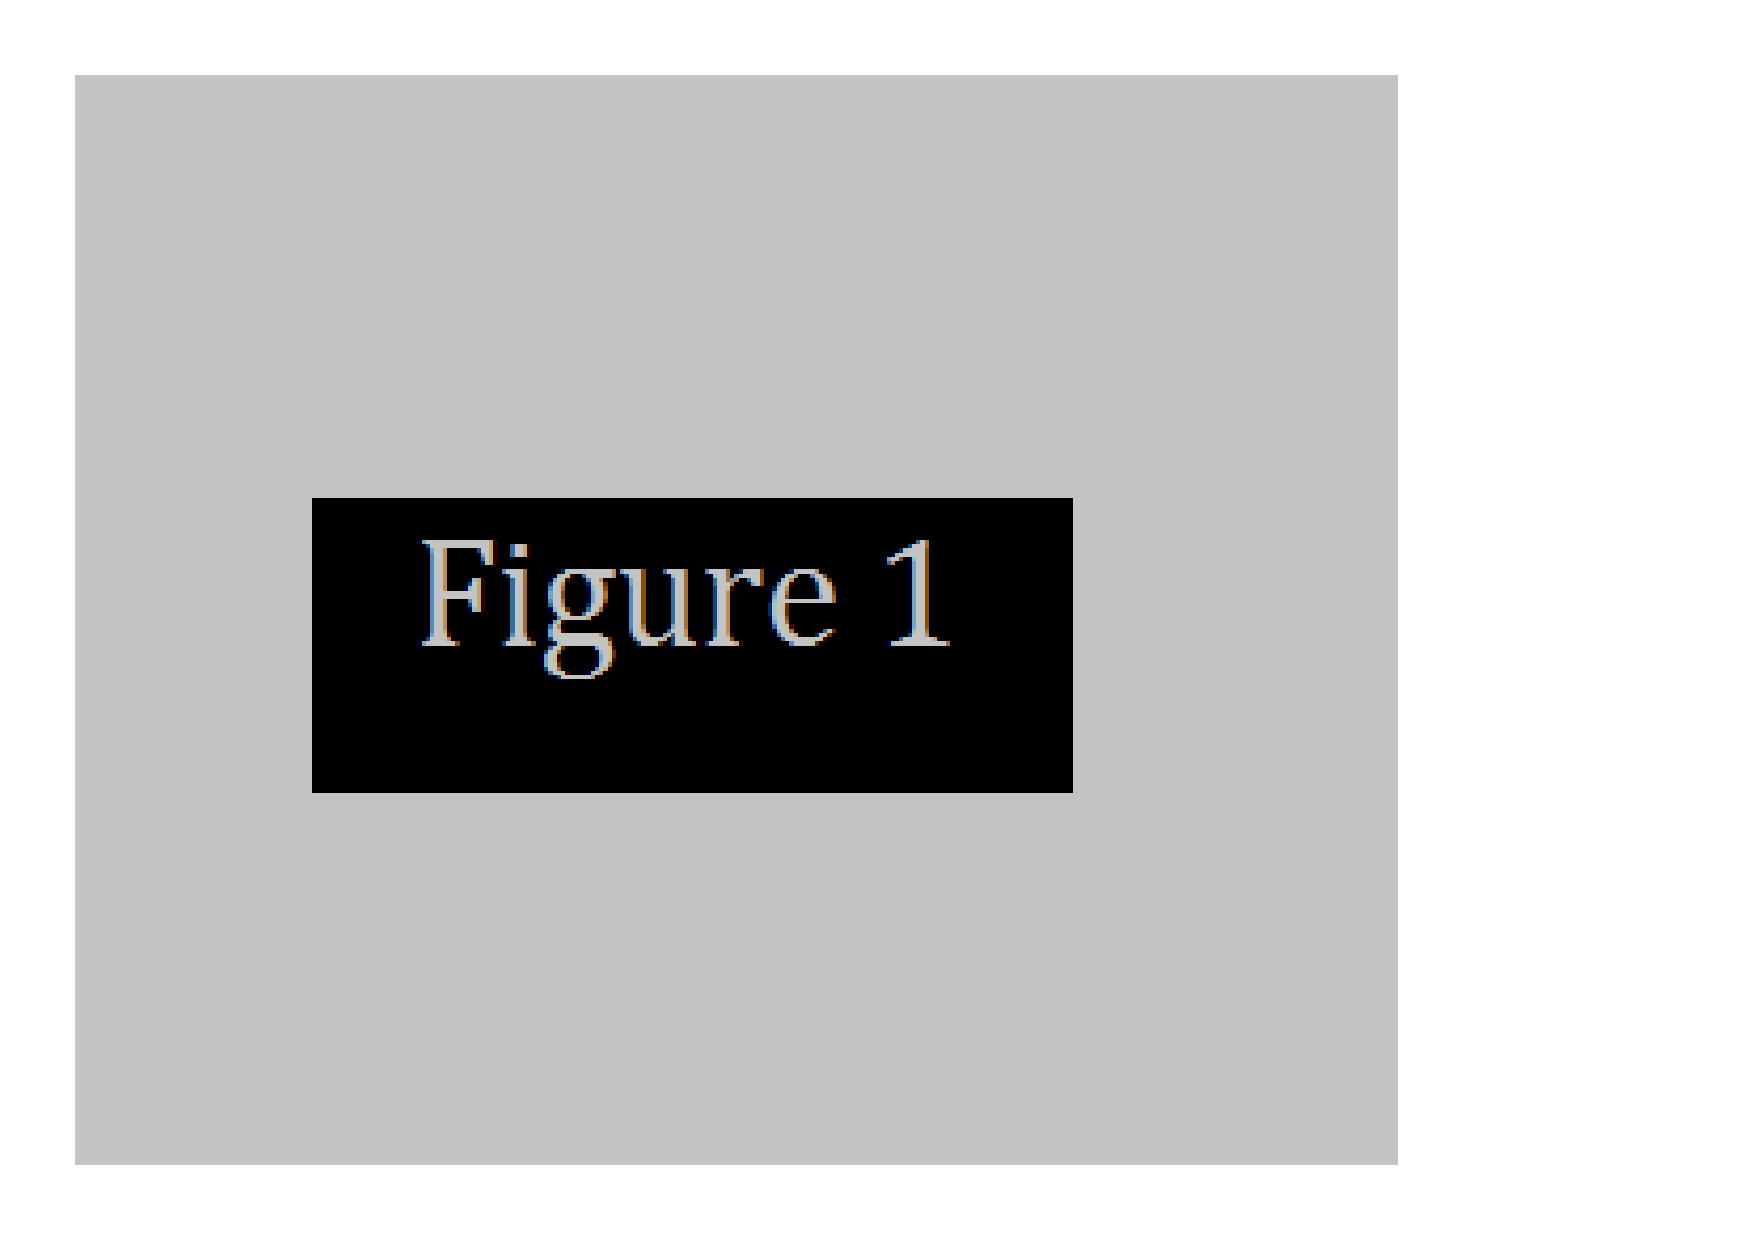
\includegraphics[width = 0.3\linewidth]{figure1.pdf}
  \caption{...}\label{fig:plot1}
\end{figure}	
\end{verbatim}
shows how to insert Figure~\ref{fig:plot1}. The option [{\ttfamily tb}] tells the compiler to place the figure at the top (first priority) or bottom (second priority) of the page. The figure can be scaled using the [{\ttfamily width}=...] option. Usually the width is specified as a fraction,  (say 0.3) of \textbackslash{\ttfamily linewidth}. This template can use *.pdf, *.png, *.jpg figures.

\begin{figure}[tb]
\centering
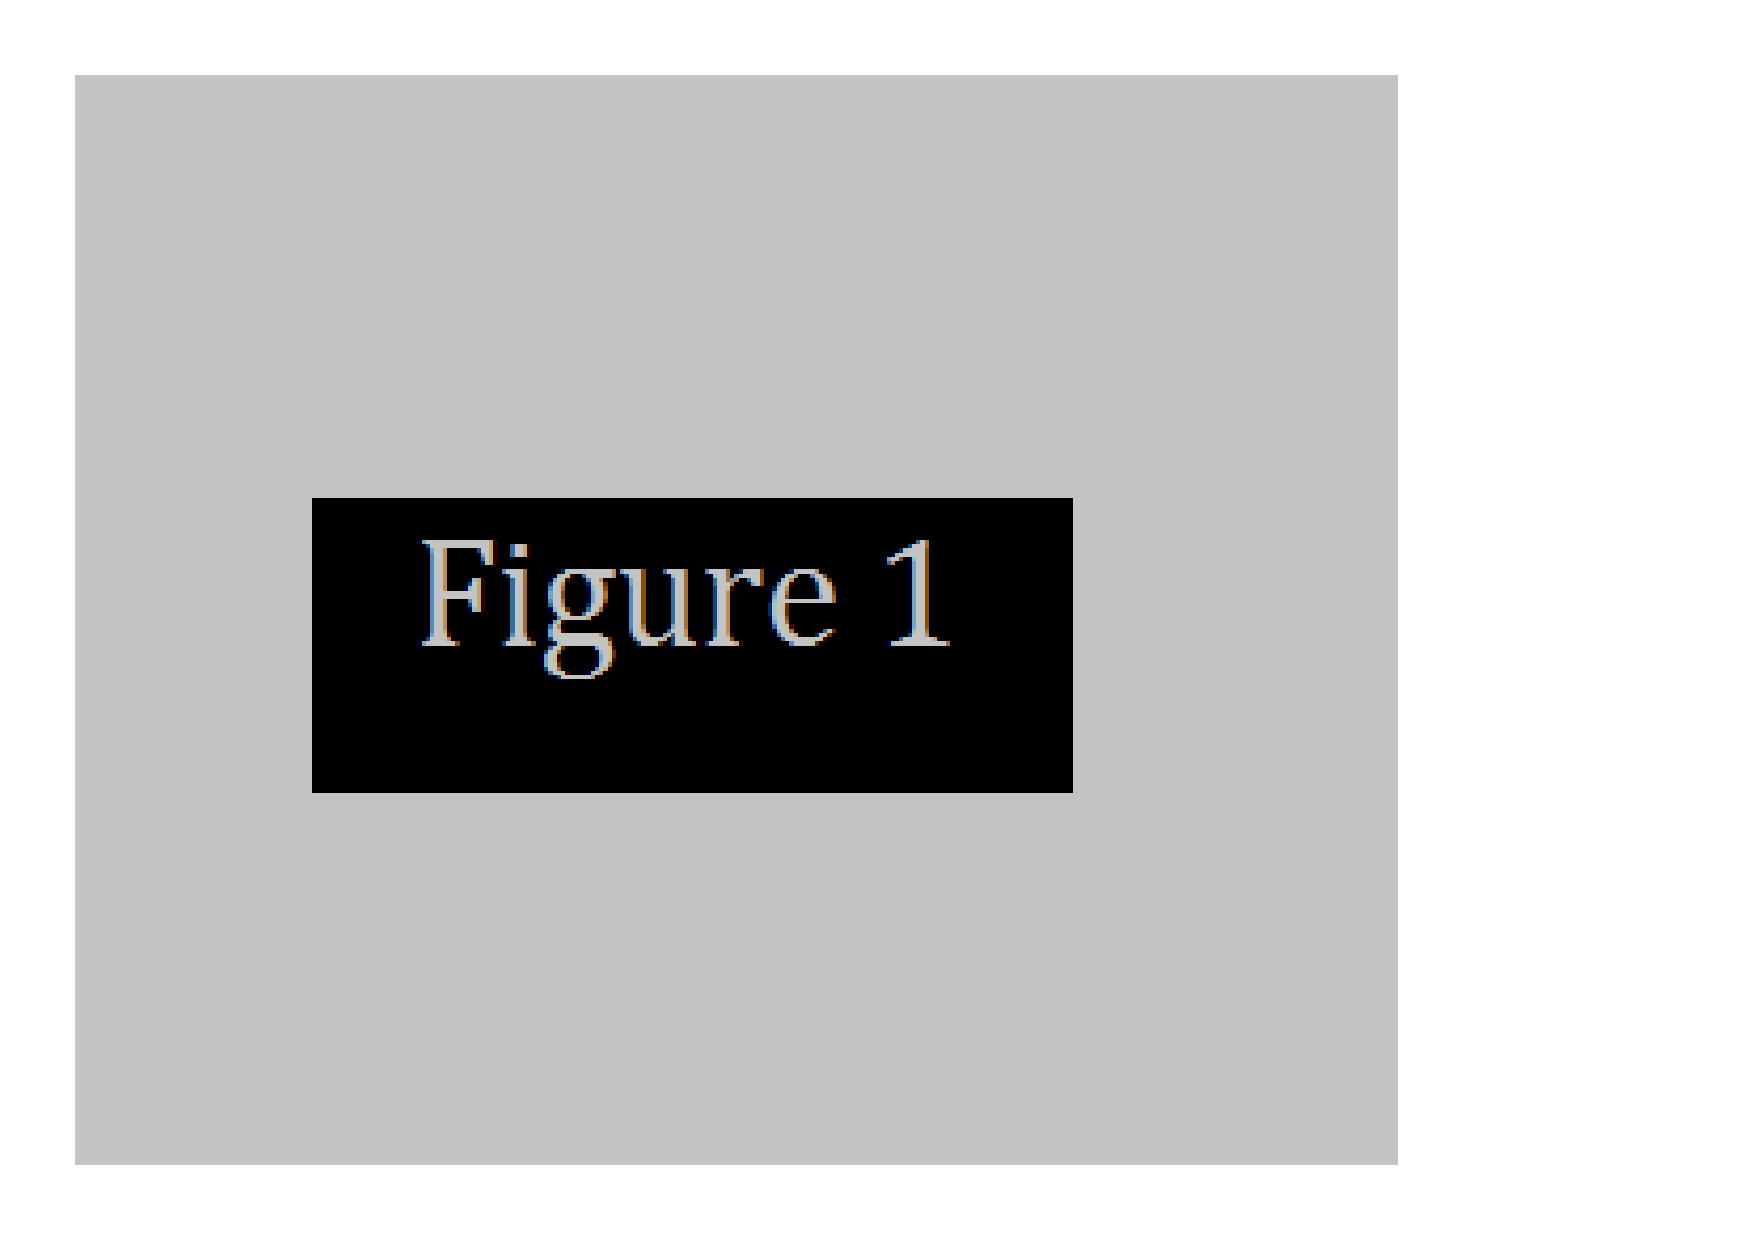
\includegraphics[width=0.3\linewidth]{figure1.pdf}
\caption{This is an example of a single column-wide figure. Figure captions are preferably self-contained and in vector format (versus raster format).}
\label{fig:plot1}
\end{figure}

Ed ut perspiciatis unde omnis iste natus error sit voluptatem accusantium doloremque laudantium, totam rem aperiam, eaque ipsa quae ab illo inventore veritatis et quasi architecto beatae vitae dicta sunt explicabo. Nemo enim ipsam voluptatem quia voluptas sit aspernatur aut odit aut fugit, sed quia consequuntur magni dolores eos qui ratione voluptatem sequi nesciunt. Neque porro quisquam est, qui dolorem ipsum quia dolor sit amet, consectetur, adipisci velit, sed quia non numquam eius modi tempora incidunt ut labore et dolore magnam aliquam quaerat voluptatem. Ut enim ad minima veniam, quis nostrum exercitationem ullam corporis suscipit laboriosam, nisi ut aliquid ex ea commodi consequatur? Quis autem vel eum iure reprehenderit qui in ea voluptate velit esse quam nihil molestiae consequatur, vel illum qui dolorem eum fugiat quo voluptas nulla pariatur?

Ed ut perspiciatis unde omnis iste natus error sit voluptatem accusantium doloremque laudantium, totam rem aperiam, eaque ipsa quae ab illo inventore veritatis et quasi architecto beatae vitae dicta sunt explicabo. Nemo enim ipsam voluptatem quia voluptas sit aspernatur aut odit aut fugit, sed quia consequuntur magni dolores eos qui ratione voluptatem sequi nesciunt. Neque porro quisquam est, qui dolorem ipsum quia dolor sit amet, consectetur, adipisci velit, sed quia non numquam eius modi tempora incidunt ut labore et dolore magnam aliquam quaerat voluptatem. Ut enim ad minima veniam, quis nostrum exercitationem ullam corporis suscipit laboriosam, nisi ut aliquid ex ea commodi consequatur? Quis autem vel eum iure reprehenderit qui in ea voluptate velit esse quam nihil molestiae consequatur, vel illum qui dolorem eum fugiat quo voluptas nulla pariatur?


\subsection{Subfigures}
To save space, multiple subfigures may also be inserted as subfloats within a single figure environment, as in Figure~\ref{fig:plots}. Here is the code:
\begin{verbatim}
\begin{figure}[tbp]
  \centering
  \subfloat{\makebox[0.4\textwidth]{\includegraphics{a.pdf}\label{fig:fa}}}
  \quad % or other spacing between figures
  \subfloat{\makebox[0.4\textwidth]{\includegraphics{b.jpg}\label{fig:fb}}}
  \caption{Multiple images can be inserted inline.}\label{fig:plots}
\end{figure}
\end{verbatim}

\begin{figure}[tbp]
  \centering
  \subfloat[Optional subcaption of this subfigure.]{\makebox[0.4\textwidth]{{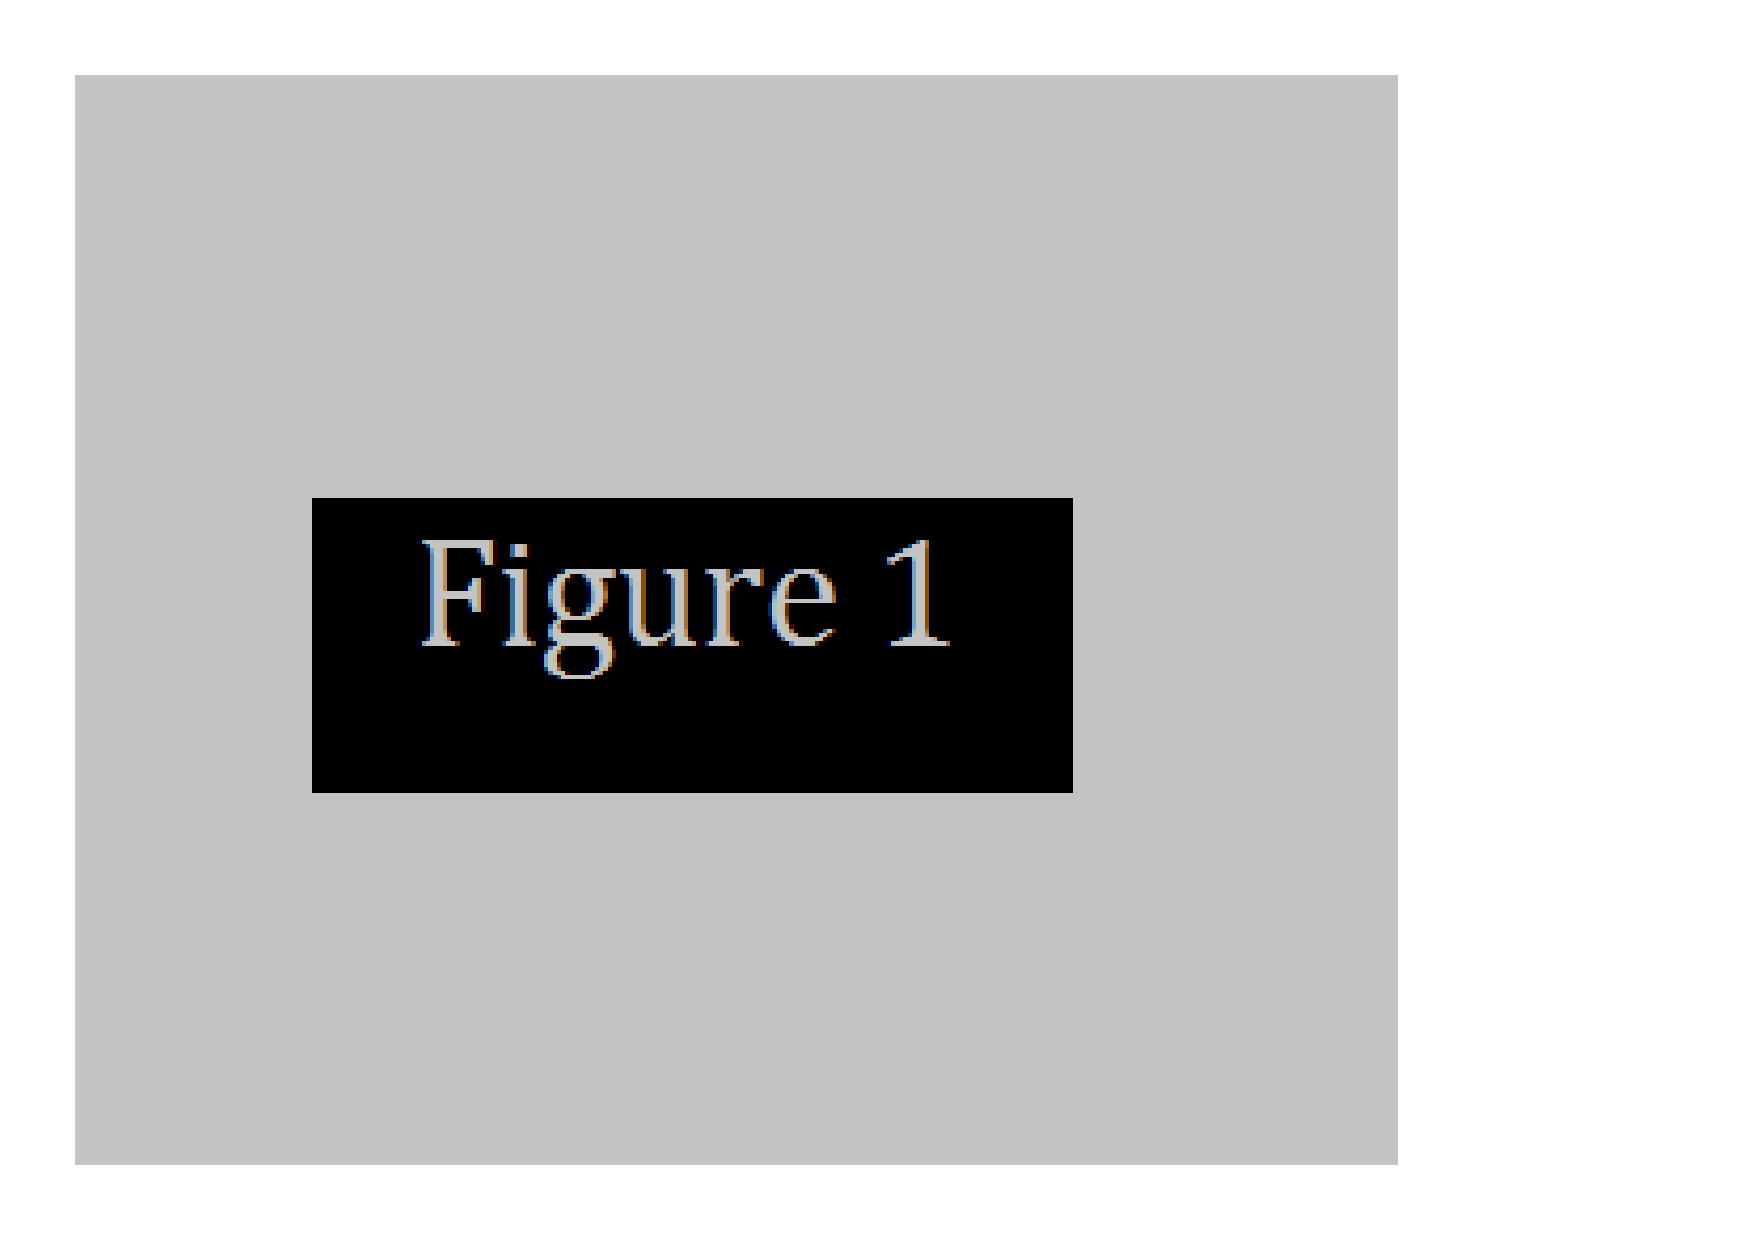
\includegraphics[width=0.2\textwidth]{figure1.pdf}\label{fig:f1}}}}
  \quad % or other spacing between figures
  \subfloat{\makebox[0.4\textwidth]{
\includegraphics[width=0.3\textwidth]{figure2.jpg}\label{fig:f2}}}
  \caption{Multiple images can be inserted inline.}\label{fig:plots}
\end{figure}


Ed ut perspiciatis unde omnis iste natus error sit voluptatem accusantium doloremque laudantium, totam rem aperiam, eaque ipsa quae ab illo inventore veritatis et quasi architecto beatae vitae dicta sunt explicabo. Nemo enim ipsam voluptatem quia voluptas sit aspernatur aut odit aut fugit, sed quia consequuntur magni dolores eos qui ratione voluptatem sequi nesciunt. Neque porro quisquam est, qui dolorem ipsum quia dolor sit amet, consectetur, adipisci velit, sed quia non numquam eius modi tempora incidunt ut labore et dolore magnam aliquam quaerat voluptatem. Ut enim ad minima veniam, quis nostrum exercitationem ullam corporis suscipit laboriosam, nisi ut aliquid ex ea commodi consequatur? Quis autem vel eum iure reprehenderit qui in ea voluptate velit esse quam nihil?

\begin{table}[b]
\centering % center-align tables within a column
\caption{This is an example of a single column table. Captions are preferably self-contained and placed above the table. Columns may be left-, center-, decimal marker-, or right-aligned.}\label{table:label1}
\begin{tabular}{l c d{2.3} r}
\toprule
Example & Count 	1			& \multicolumn{1}{c}{Count 2} & Total\\
\midrule
A 						& 2.345 					& 5.435 																		& 16.78(3)\\
B 						& 3.0 							& 12.0																				& 43.2(5)\\
\bottomrule
\end{tabular}
\end{table}

\subsection{Tables}
In the sample Table~\ref{table:label1} the environment
\begin{verbatim} 
\begin{table}
\centering 
\caption{...}
 \begin{tabular}{l c d{2.3} r}
   \toprule
   ... & ... & ... & ... \\
   \midrule
   ... & ... & ... & ... \\
   \bottomrule
 \end{tabular}
\end{table}
\end{verbatim} 
constructs a four-column table with the first column left-aligned, second column centered, third column aligned on the decimal point with 2 integer digits and 3 decimal places, and the fourth column right-aligned. Ampersands {\ttfamily \&} separate columns while double backslashes \textbf{\textbackslash\textbackslash} \ start a new row.

Ed ut perspiciatis unde omnis iste natus error sit voluptatem accusantium doloremque laudantium, totam rem aperiam, eaque ipsa quae ab illo inventore veritatis et quasi architecto beatae vitae dicta sunt explicabo. Nemo enim ipsam voluptatem quia voluptas sit aspernatur aut odit aut fugit, sed quia consequuntur magni dolores eos qui ratione voluptatem sequi nesciunt. Neque porro quisquam est, qui dolorem ipsum quia dolor sit amet, consectetur, adipisci velit, sed quia non numquam eius modi tempora incidunt ut labore et dolore magnam aliquam quaerat voluptatem. Ut enim ad minima veniam, quis nostrum exercitationem ullam corporis suscipit laboriosam, nisi ut aliquid ex ea commodi consequatur? Quis autem vel eum iure reprehenderit qui in ea voluptate velit esse quam nihil molestiae consequatur, vel illum qui dolorem eum fugiat quo voluptas nulla pariatur?

\section{Using BibTeX for the References}
The included BibTeX file {\ttfamily bibfile}.{\ttfamily bib} contains several sample entries. BibTeX formatted citations are easily downloadable from search engines. Please use standard journal abbreviations. As much as possible, do include the {\ttfamily DOI}=\{{\ttfamily 10.XXXX}/{\ttfamily XXXX}\}{\ttfamily ,} entry so that references are automatically hyperlinked (\textbf{do not include} the leading {\ttfamily http}:\textbackslash\textbackslash{\ttfamily dx.doi.org}\textbackslash).

For a journal article, the recommended fields to be filled in are
\begin{verbatim}
@article{articlekey,
title={...},
author={Full Surname Sr., First N. and ...},
journal={J. Abbrev.},
volume={33},
pages={555},
year={2016},
doi={10.1000/num.1000}
}
\end{verbatim}
Each author is separated by the word {\ttfamily and}. Suffixes are attached to the author last name.

For Proceedings and Conference Articles, several examples are given {\ttfamily bibfile}.{\ttfamily bib} \cite{proceedingskey1,proceedingskey2}.

\section{Conclusions}
Here is the Summary or Conclusions section.

\section*{Acknowledgments}
Here are the acknowledgments. Note the asterisk \textbackslash{\ttfamily section*}\{{\ttfamily Acknowledgments}\} that signifies that this section is unnumbered.

\section*{*Additional Reminders}
\begin{itemize}
    \item The most common cause of manuscript processing delays is incorrect formatting of the (1) author block and affiliation bylines, and (2) references. Please verify that all blue web hyperlinks resolve correctly.
    \item The Full Proceedings is also prepared in print. Please follow the maximum page limit of Four (4) pages \textit{including references}. 
\end{itemize}

% Please use the style file spp-bst.bst. If you wish to use BibTeX, kindly use us the filename bibfile.bib for your bib file.
\bibliographystyle{spp-bst}
\bibliography{bibfile}

\end{document}